\chapter{Tactile Sensing} \label{Chapter:TactileSensing}
The tactile sensing fabricated and used in this research took inspiration from examples seen in the literature \cite{First3DHall,James}. It uses the hall effect to monitor the relative position of a hall effect sensor and a magnet. The magnets are embedded in a silicon rubber such that contact with the rubber will cause a deformation and a proportional change in magnet-sensor relative position. Magnets are embedded in silicon and placed over a hall effect sensor. An air gap between sensor and silicon is used to increase sensitivity \cite{HSSoft}.

\section{Material}
The material used was a "Polycraft T-15 Translucent Silicon Rubber" \cite{Silicon}. It is described by the manufacturer as a "two-component, high strength, flexible, moulding compound". It was found to be suitable for this application, since it is sufficiently robust so as to not deteriorate or change in performance after successive collisions during testing. It is sufficiently flexible, and of a suitable elasticity to act as a medium to suspend the magnet in such that a small force contacting the surface causes a detectable change in the relative sensor-magnet position. Finally, since it was a two-part compound it was easy to mould to a custom shape. The silicon remained liquid until and for approximately 20 mins after the two parts where mixed. This was sufficient time to fill and close the mold.

\section{Sensor}
The sensor used was an MLX90393 hall effect sensor \cite{MLX}. This particular sensor is highly suitable for this application and for this reason can also be seen in prior literature. The sensor is:
\begin{itemize}
    \item Small
    
    The MLX90393 is 3x3x1mm. This is particularly important since the tactile sensing is implemented onto the tip of a robotic gripper which is a size comparable to that of a human hand.
    \item Simple to implement
    
    The sensor itself has a lot of built in logic and can be interfaced with via the I2C communication protocol, making it simple to implement. Parameters such as the sample frequency, mode (burst, single measurement and wake-on-change), sensitivity, gain, etc. can be set and data collected using an appropriate microcontroller. Furthermore the I2C communication protocol allows two communication lines (SCL and SDA) to enable communication between many devices using 7-bit addressing. This reduces the number of wires which require routing through the gripper. This presents a significant advantage since the gripper has many joints which makes routing difficult and any gripper may have a large number of tactile sensors.
    \item High Sensitivity
    
    $0.294 \frac{\mu T}{LSB}$ is stated as the maximum sensitivity of the sensor (in the Z-axis). This is orders of magnitude too sensitive for this application and causes the 16 bit long reported data to overflow such that there are discontinuities in the sensor data over the range of reasonable contact forces. To overcome this both the on-chin gain and sensitivity are set lower so as the output is within a suitable range for the application. 
    \item Mutil-axis
    
    The sensor in question reports the magnetic field strength in all three axis (X, Y and Z). This is incredibly useful for tactile sensors implemented in a robotic gripper since it has the ability to report more than just forces perpendicular to the gripper but can also infer information about shear and non-normal forces. Theoretically this would give a gripper the ability to infer an objects weight, and surface characteristics as well as detect slippage and the angle of incidence of a collision to name a few examples. 
    
    \item High Frequency
    
    Since this project is exploring the grasping of moving objects the ability to sample sensors at a high frequency is of upmost importance. The sample frequency of this sensor is dependant on a number of variables and settings including the sensor mode, relevant axis, BURST\_DATA\_RATE, temperature, over-sample-rate of the ADC, etc. For this reason it is difficult to give a value for the max sample rate however it is in the order of tens of milliseconds per sample or 10-100Hz.
\end{itemize}

\section{Air-gap}
One feature of the design of the tactile sensors taken directly from prior literature is the use of an air gap between the sensor and magnet-silicon. An observation both from early stage testing of a prototype sensor and from the literature is that there is significant amount of cross talk between the axis when the silicon is deformed. Cross talk is when a force normal to the surface (in the z-axis) would cause significant changes in the magnetic field in the x and/or y axis. It was discovered that the mechanism causing this cross-talk was because the silicon was elastic but relatively incompressible. Therefore when a force would deform the compliant covering, the magnet would move both in the direction of the force but also in a direction perpendicular to the force because of the flow of the material. The solution to this was to add an air gap above the sensor. Since air is compressible, and also free to flow out of the cavity, the relative movement between magnet and sensor was more representative of the force causing the deformation. Furthermore the addition of an air gap significantly increased the sensitivity of the senors. The one downside of the air gap is the increased hysteresis, however this is not an issue in the application of grasping a moving object and so will not be a problem during the course of this research.

\begin{figure}
    \centering
    \begin{subfigure}{.45\linewidth}
        \centering
 %   
\includegraphics[width=.4\textwidth]{Images/placeholder.png}       
    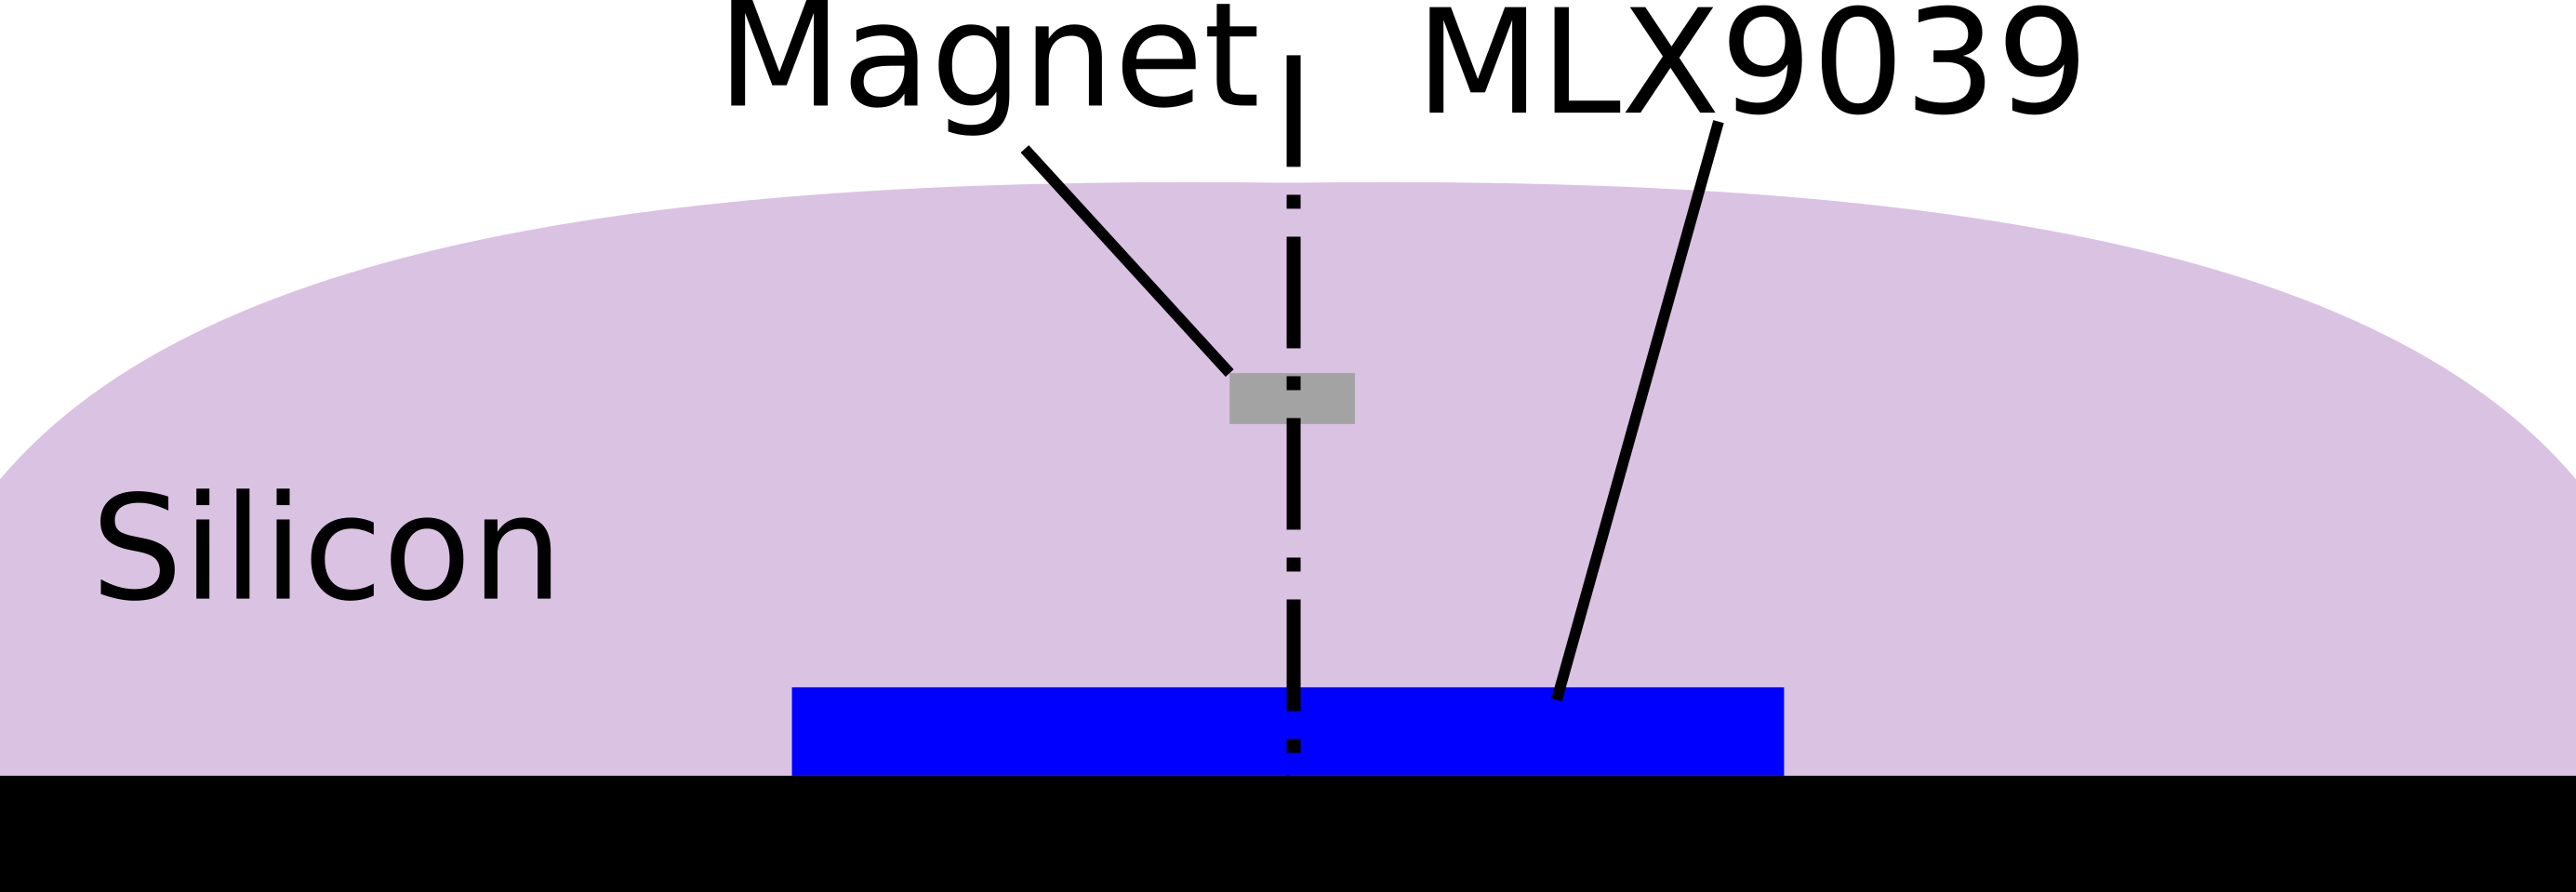
\includegraphics[width=0.7\textwidth]{Images/nogap.png}
        \caption{Without an air gap}
        \label{fig:nogap}
    \end{subfigure}
    \begin{subfigure}{.45\linewidth}
        \centering
        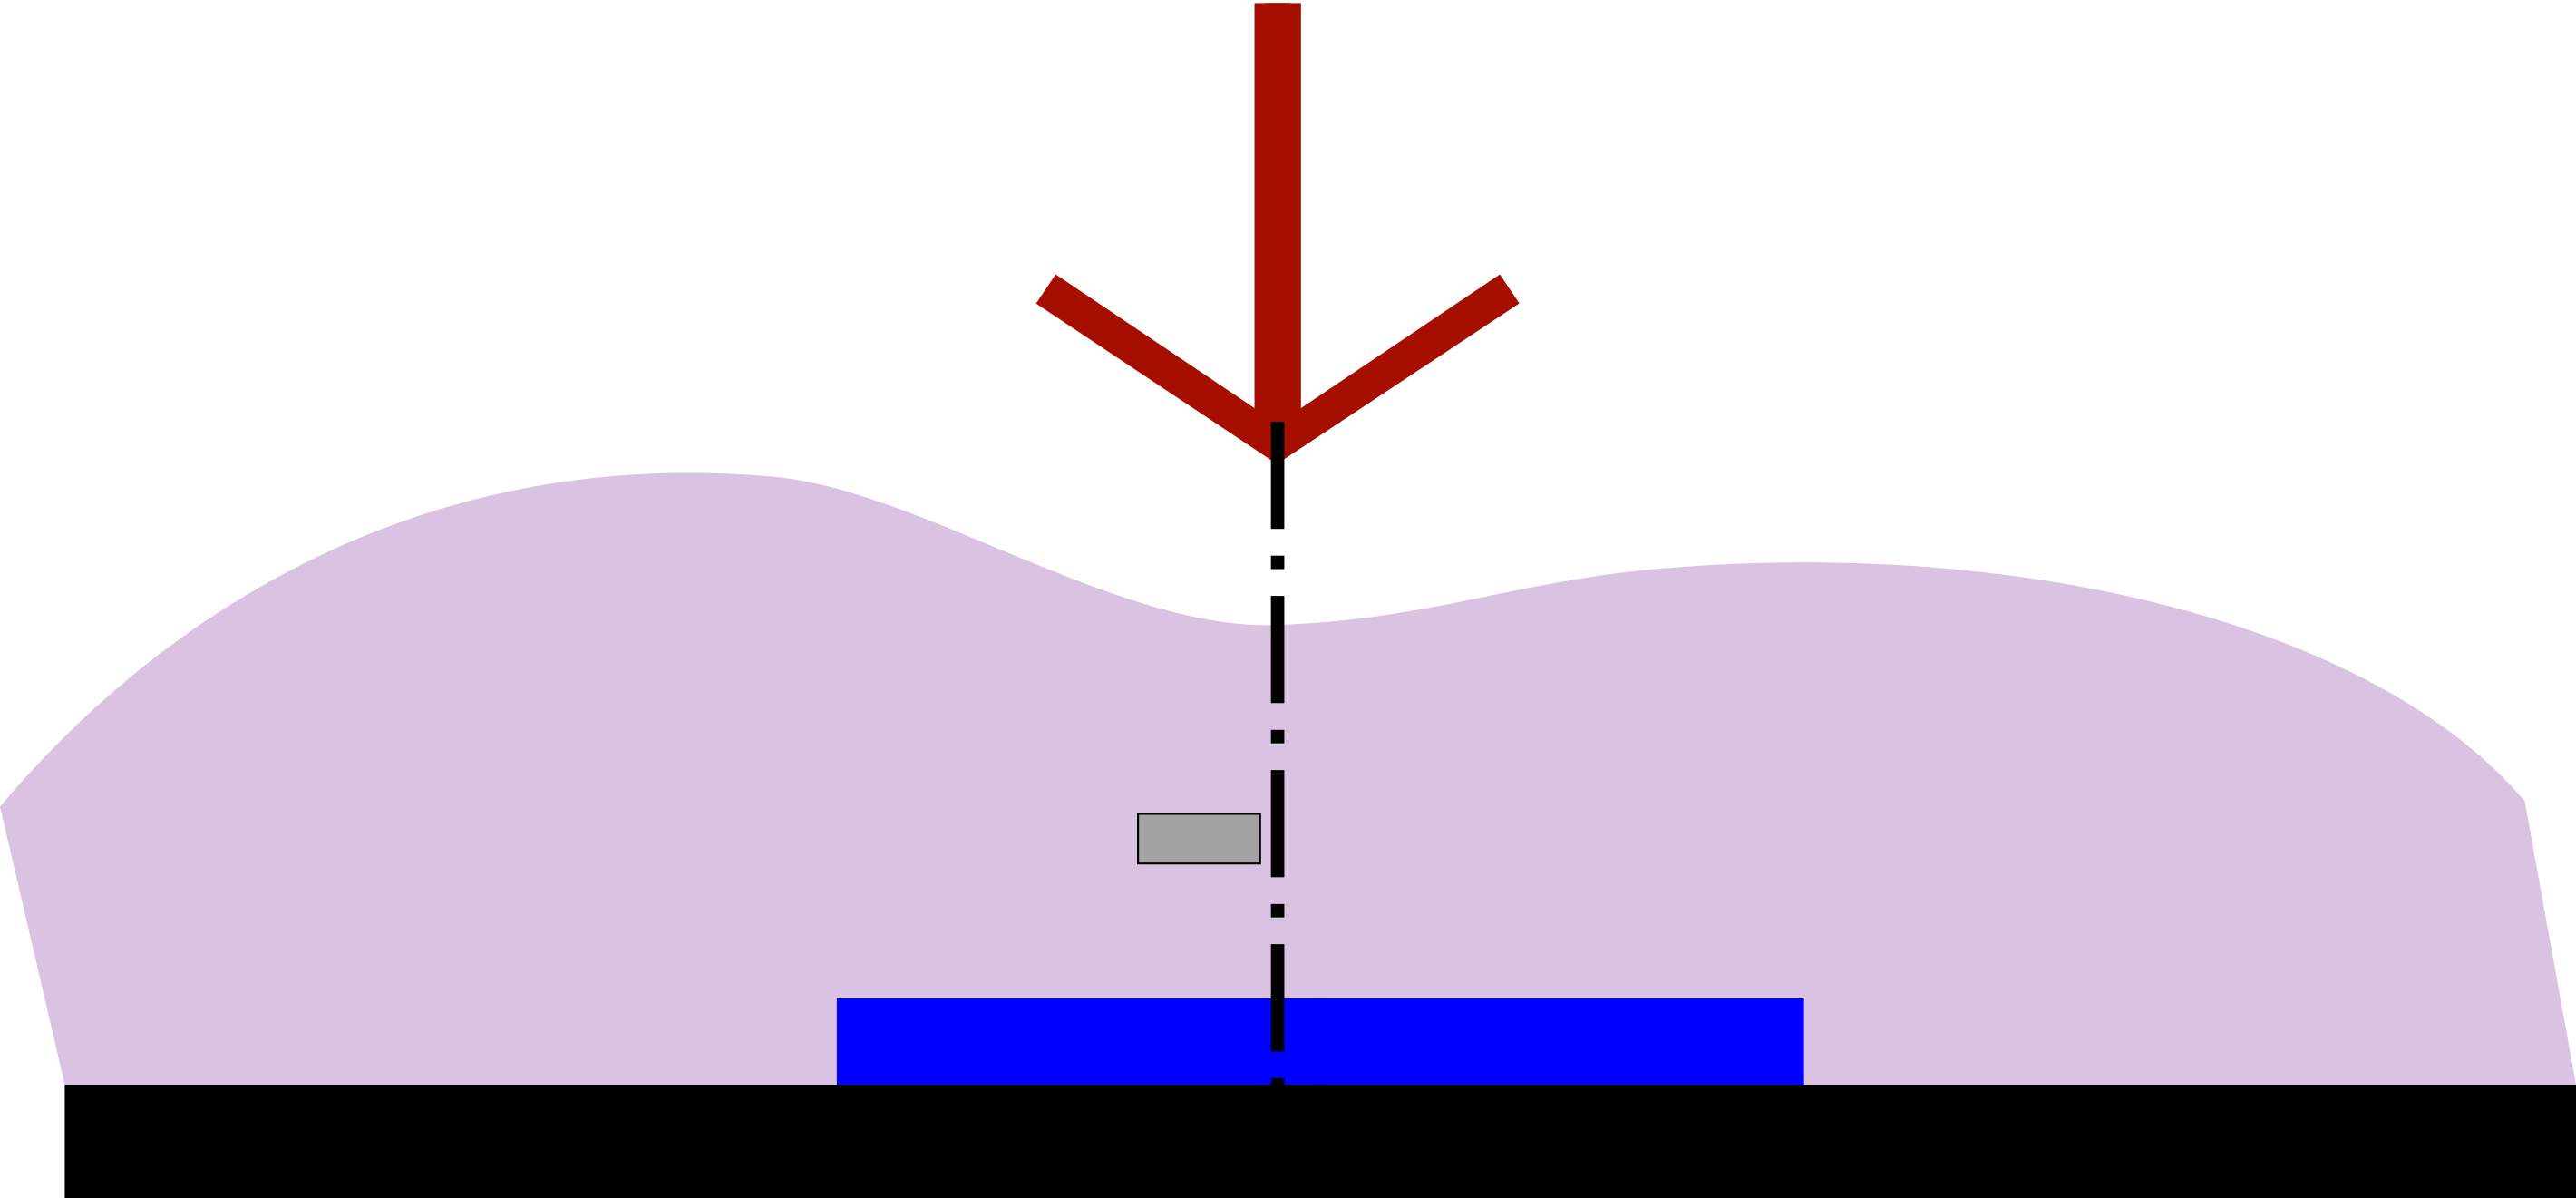
\includegraphics[width=0.7\textwidth]{Images/nogapforce.png}
%    
\includegraphics[width=.4\textwidth]{Images/placeholder.png}
        \caption{Incomprehensibility causes unpredictable material flow }
        \label{fig:nogapforce}
    \end{subfigure}
    \begin{subfigure}{.45\linewidth}
        \centering
%    
\includegraphics[width=.4\textwidth]{Images/placeholder.png}       
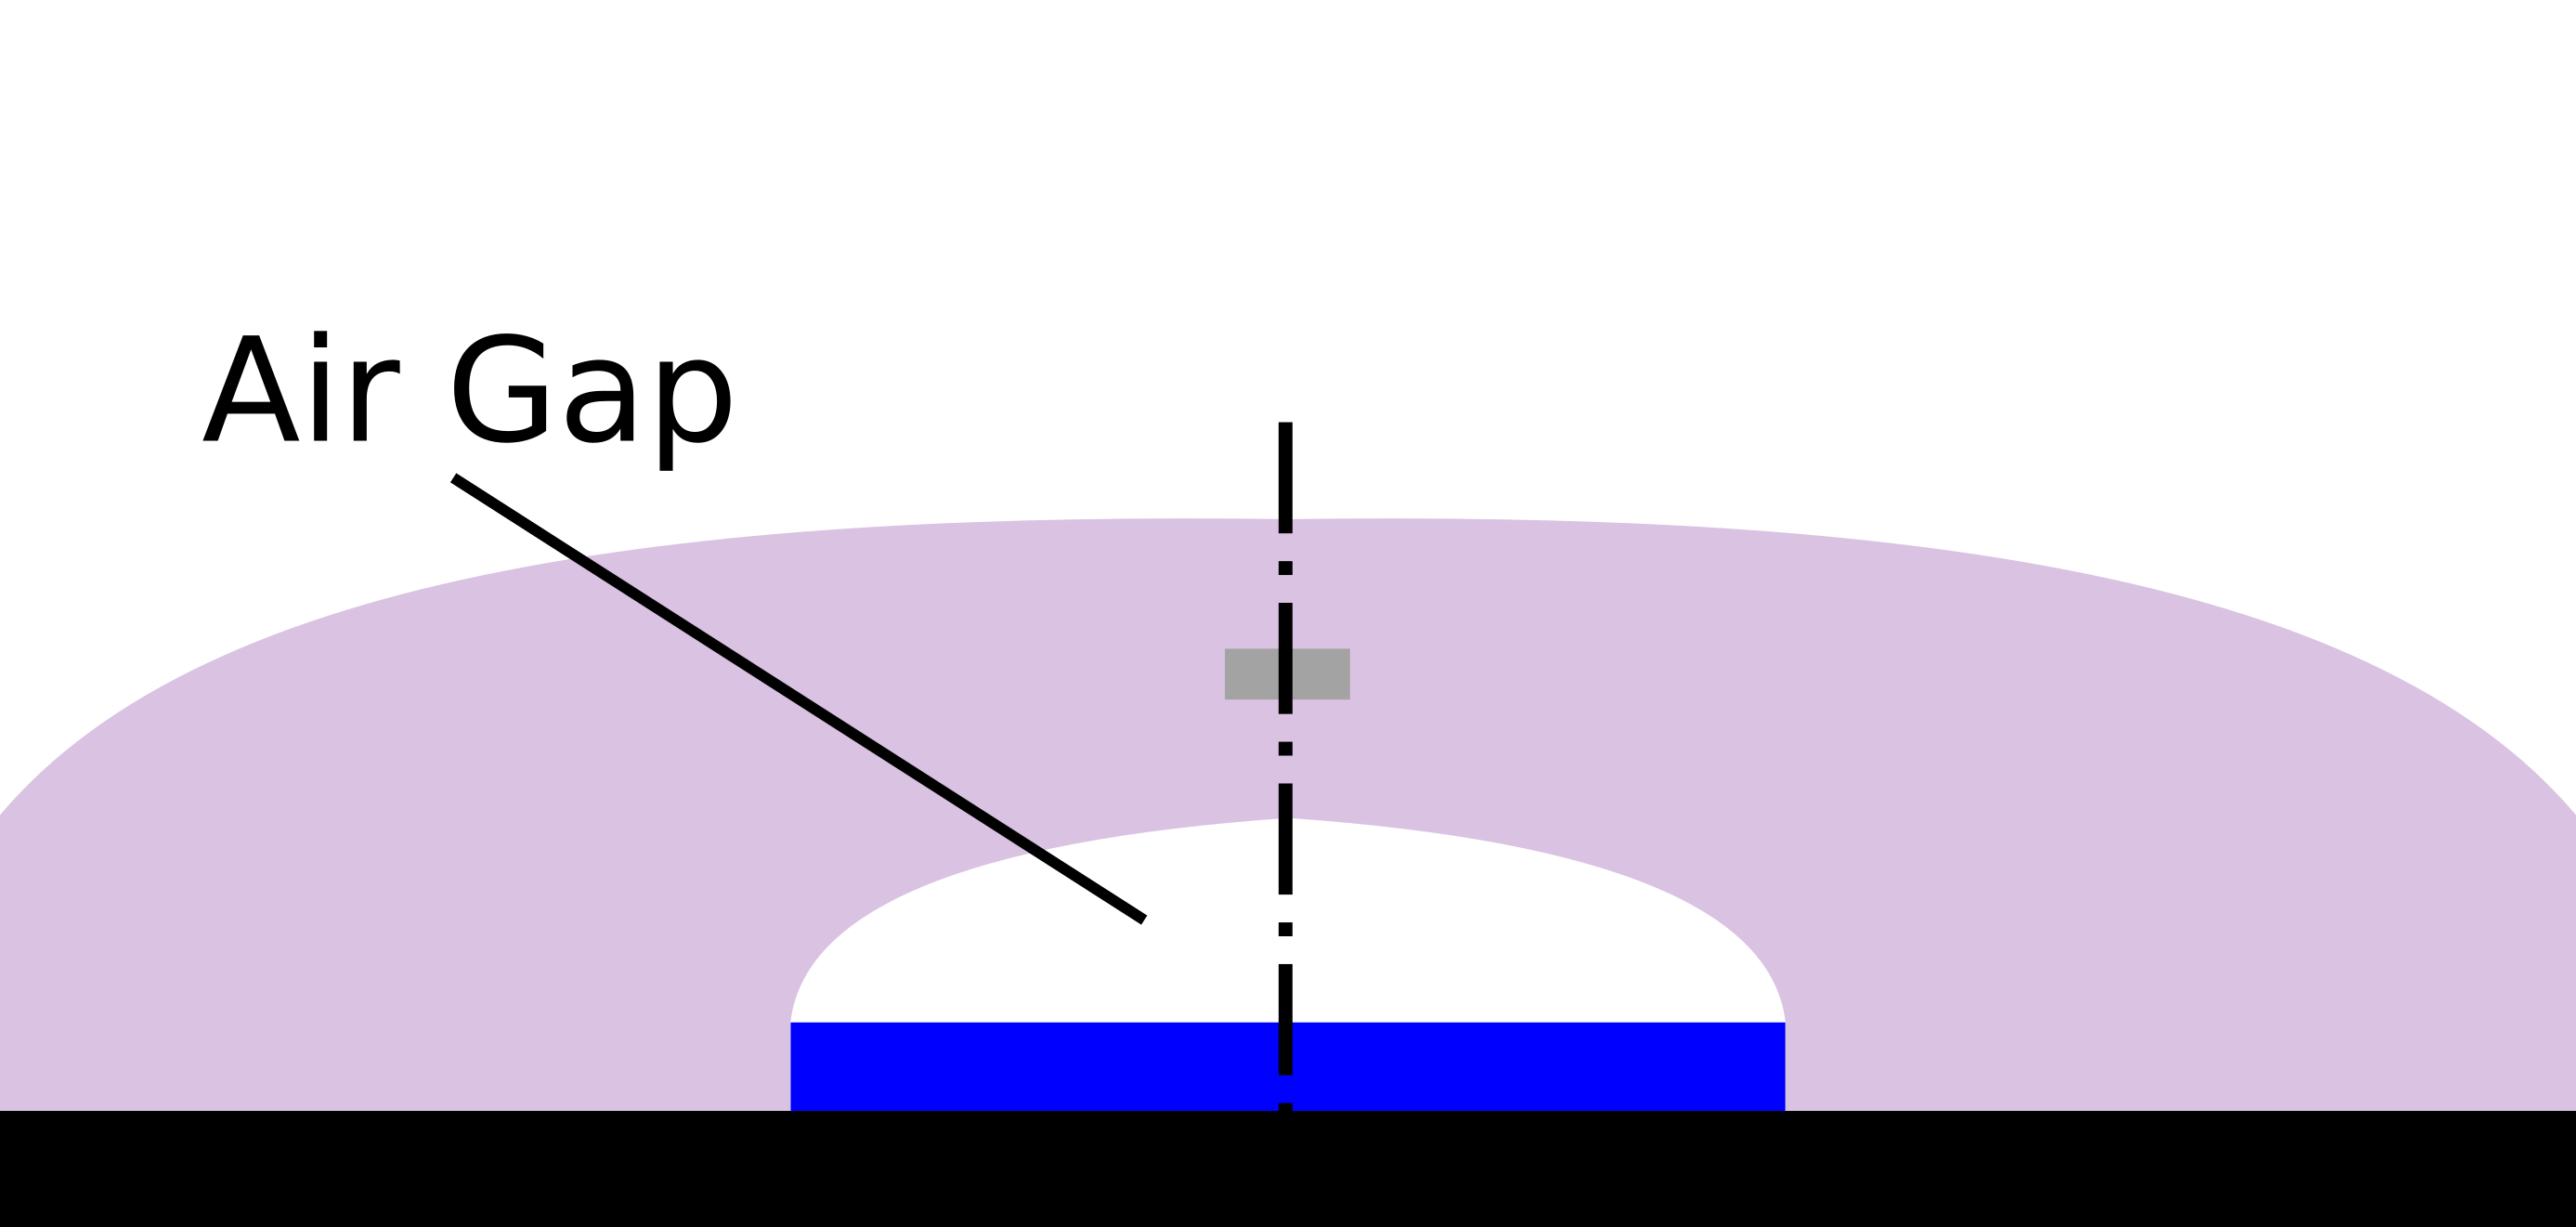
\includegraphics[width=0.7\textwidth]{Images/Airgap.png}
        \caption{Introduction of an air gap}
        \label{label:airgap}
    \end{subfigure}
    \begin{subfigure}{.45\linewidth}
        \centering
        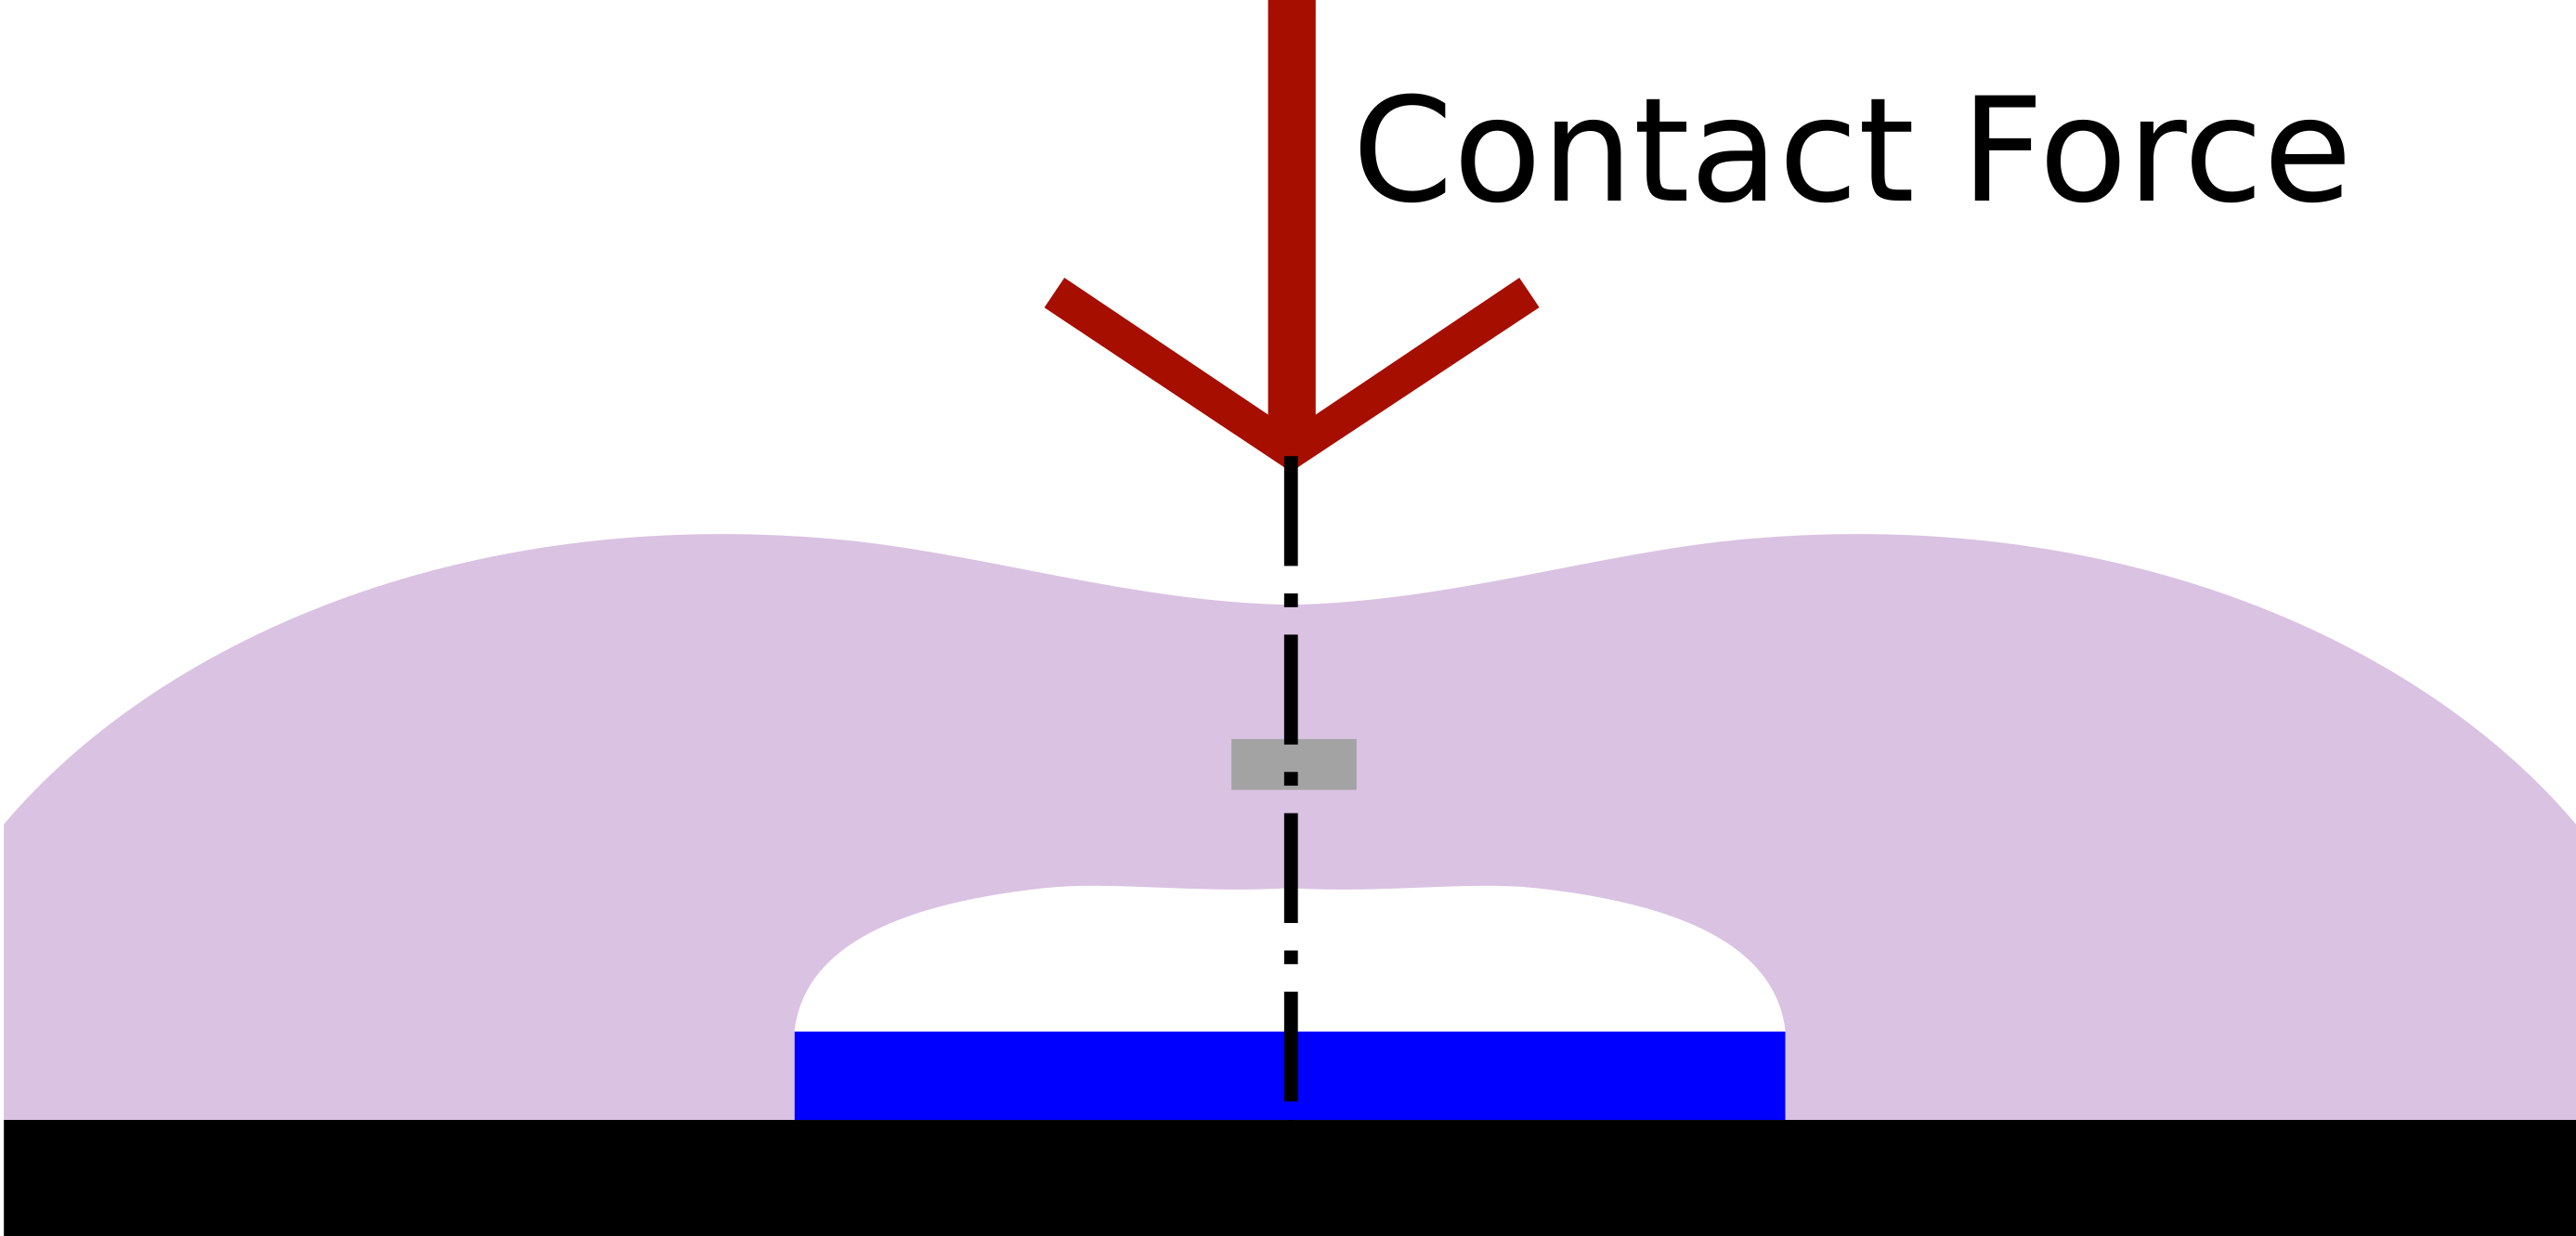
\includegraphics[width=0.7\textwidth]{Images/airgapforce.png}          
%    
\includegraphics[width=.4\textwidth]{Images/placeholder.png} 
        \caption{Displacement is in direction of the contactforce}
        \label{label:airgapforce}
    \end{subfigure}
    \label{figure:airgap}
    \caption{Shows the reason for cross-talk and the advantage of an air gap above the sensor}
\end{figure}

\section{Fabribation}
The sensor required two main fabrication methods, the printing of the PCB and the molding of the silicon rubber. The PCB, seen in Figure \ref{fig:PCB}, is a custom PCB which enables the I2C communication protocol and minimises all other wires. The manufacturing of this part was outsourced. 

The silicon was molded to a custom shape. To achieve this, molds where created from PLA using additive manufacturing, shown in Figures \ref{figure:moldCAD} \& \ref{figure:Molding}. The mold was made in two parts, the primary mold and a lid. The lid could be bolted into place and included the geometry to create an air gap and auto-alignment with the primary mold. The lid also had risers to allow excess silicon to flow out of the mold, ensuring that there were no unintentional air bubbles left in the silicon during the curing process. In order to hold the magnet in position during the curing process a small (1mm) drill bit was used to bore a hole in the bottom of the mold. The magnet could then to attached to the top of the drill bit and the drill bit friction fitted into place.

\begin{figure}
    \centering
    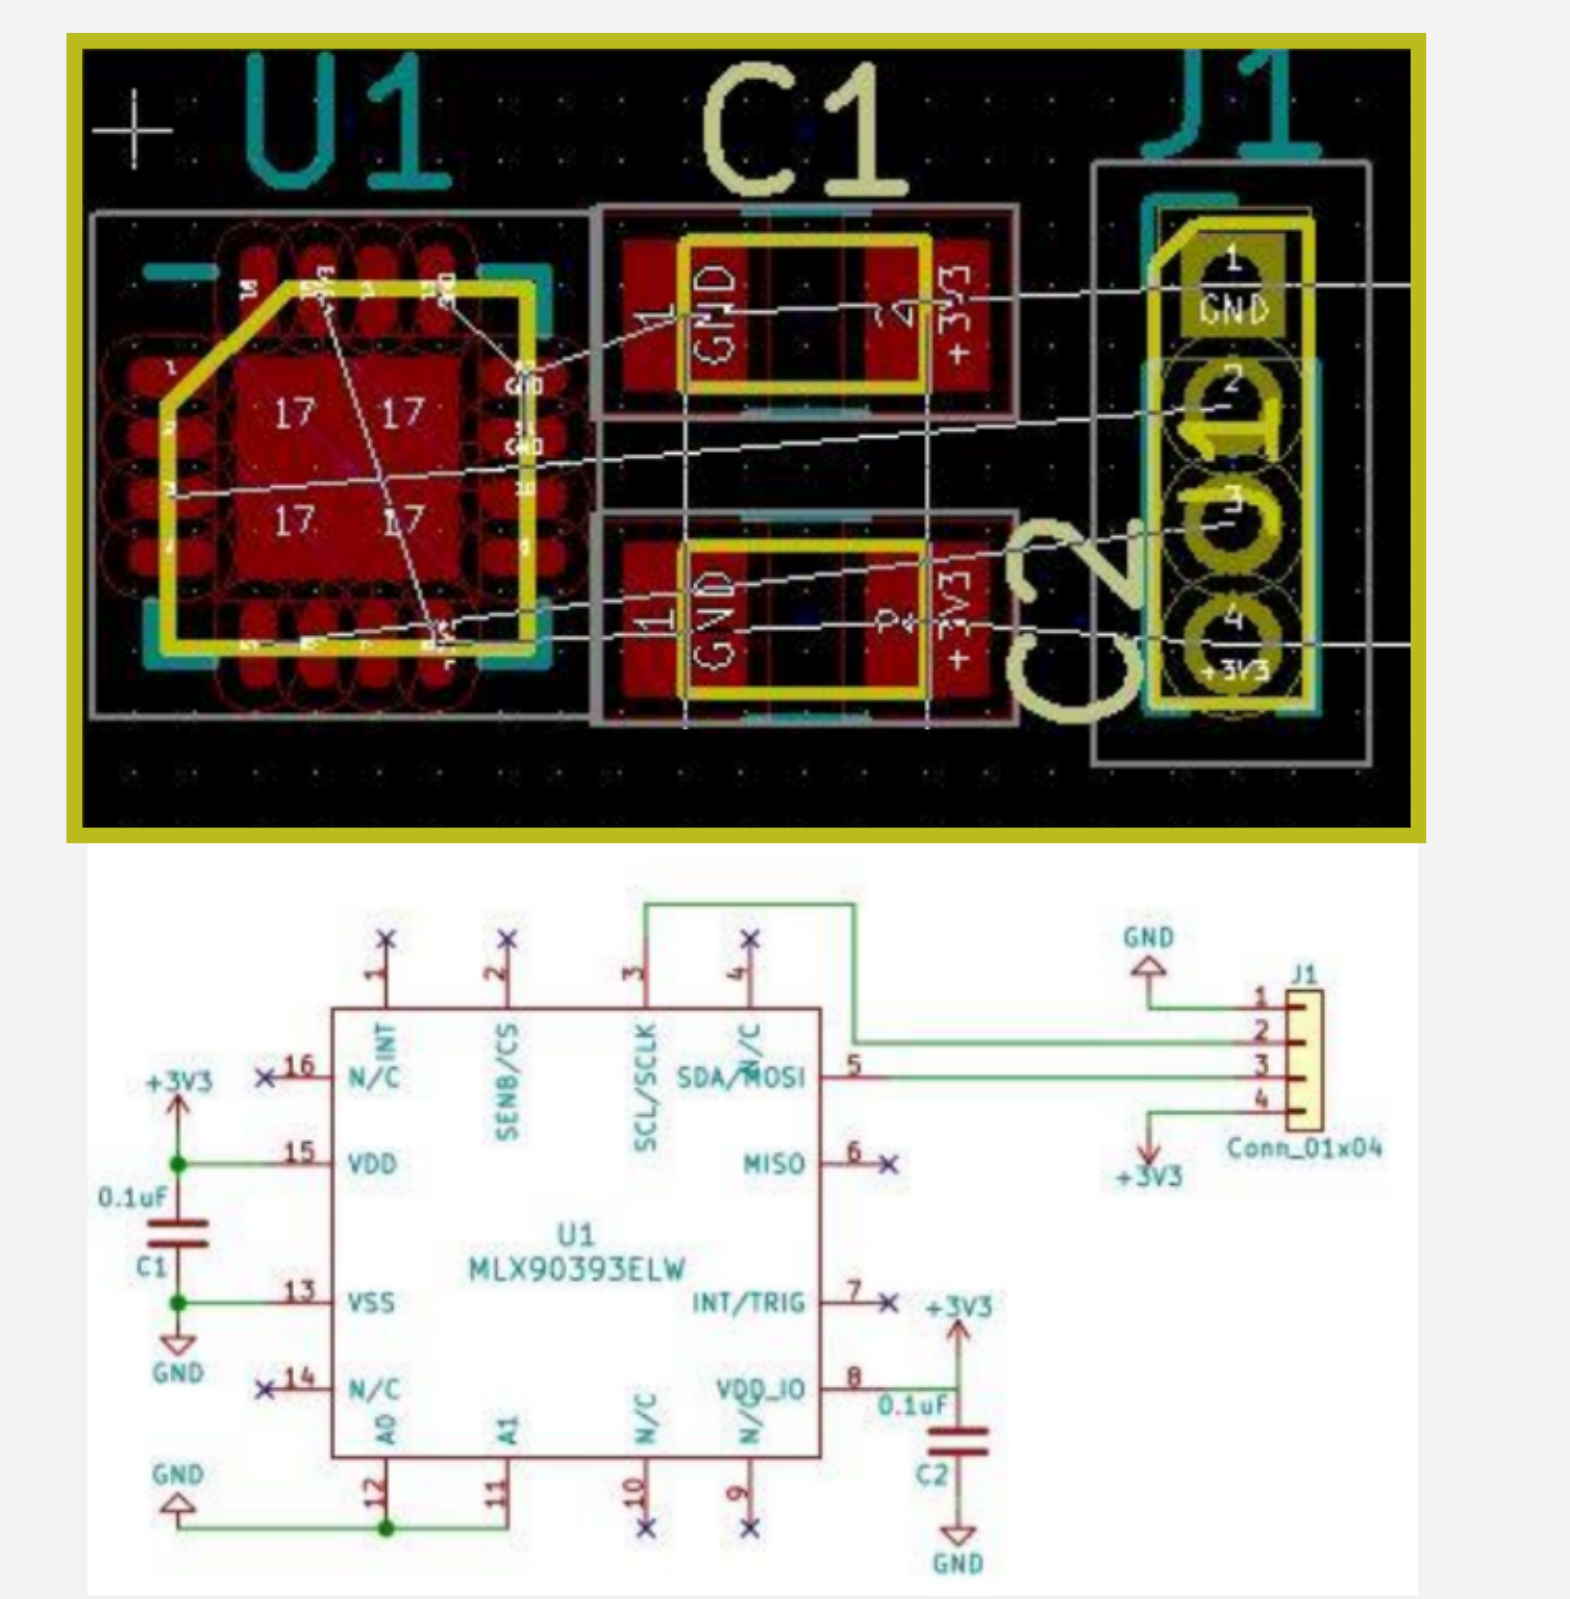
\includegraphics[width=0.7\textwidth]{Images/PCB.png}
    \caption{MLX90393 PCB}
    \label{fig:PCB}
\end{figure}

\begin{figure}
    \centering
    \begin{subfigure}{.3\linewidth}
        \centering
 %   
\includegraphics[width=.4\textwidth]{Images/placeholder.png}       
    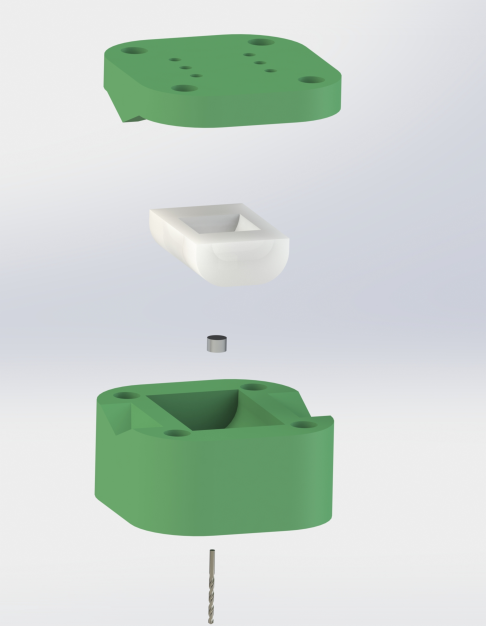
\includegraphics[width=0.7\textwidth]{Images/mold/exploded.png}
        \caption{Exploded View}
        \label{fig:exploded}
    \end{subfigure}
    \begin{subfigure}{.3\linewidth}
        \centering
%    
\includegraphics[width=.4\textwidth]{Images/placeholder.png}       
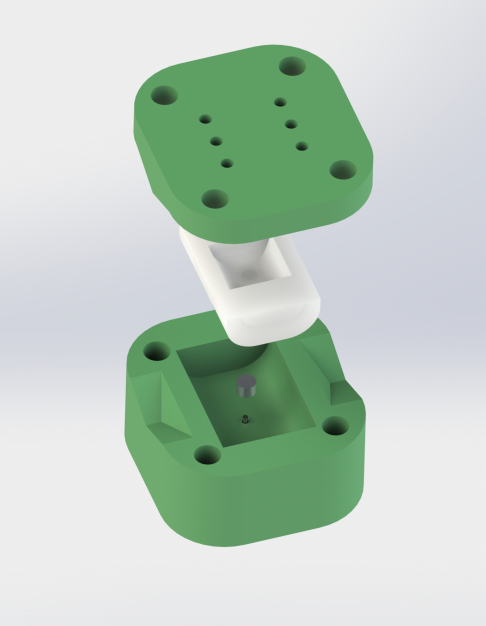
\includegraphics[width=0.7\textwidth]{Images/mold/magnetoff.png}
        \caption{Drillbit in place}
        \label{label:Drillbitinplace}
    \end{subfigure}
    \begin{subfigure}{.3\linewidth}
        \centering
        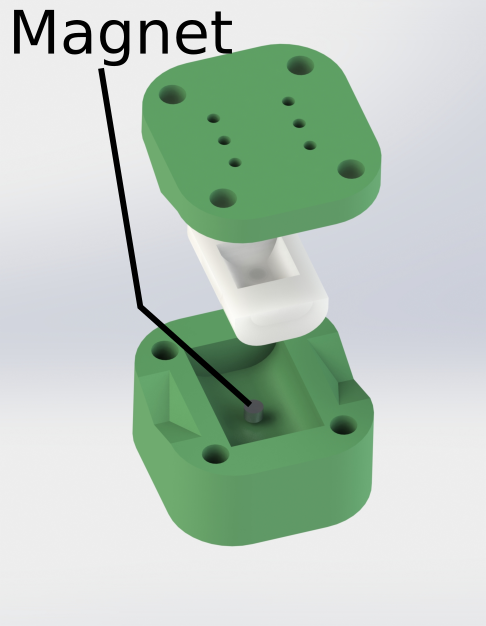
\includegraphics[width=0.7\textwidth]{Images/mold/siliconout.png}          
%    
\includegraphics[width=.4\textwidth]{Images/placeholder.png} 
        \caption{Magnet in place}
        \label{label:magnetinplace}
    \end{subfigure}
    \begin{subfigure}{.3\linewidth}
        \centering
        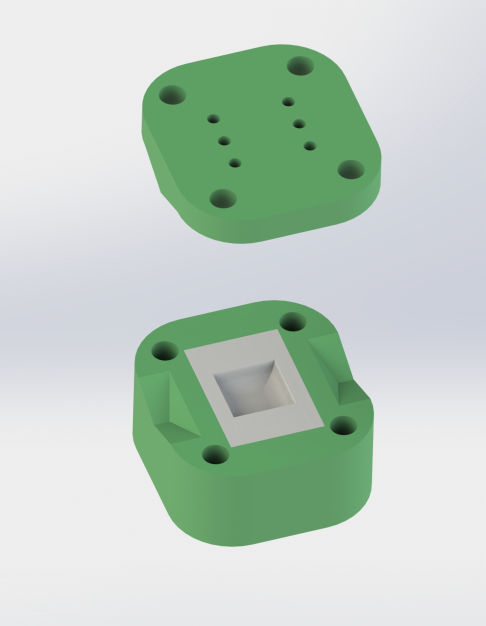
\includegraphics[width=0.7\textwidth]{Images/mold/lidoff.png}       
  %  
\includegraphics[width=.4\textwidth]{Images/placeholder.png}
        \caption{Lid off}
        \label{fig:LidOff}
    \end{subfigure}
        \begin{subfigure}{.3\linewidth}
        \centering
        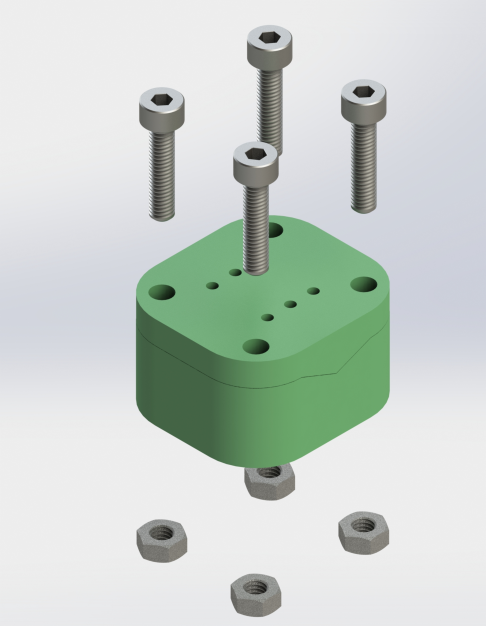
\includegraphics[width=0.7\textwidth]{Images/mold/unbolted.png}
%    
\includegraphics[width=.4\textwidth]{Images/placeholder.png}
        \caption{Bolted, to compress the mold}
        \label{fig:unbolted}
    \end{subfigure}
    \begin{subfigure}{.3\linewidth}
        \centering
        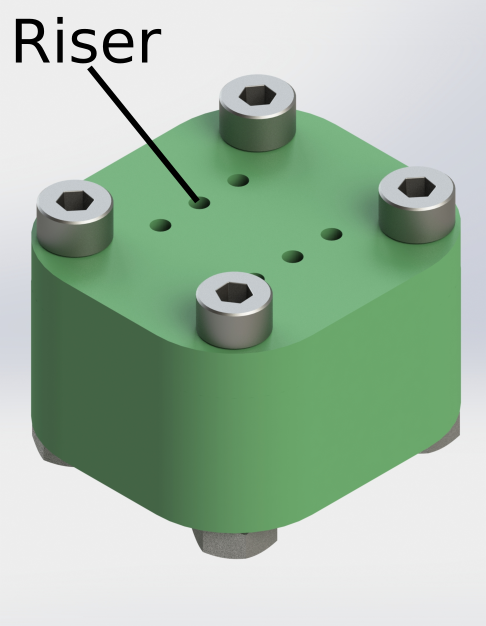
\includegraphics[width=0.7\textwidth]{Images/mold/bolted.png}    
  %  
\includegraphics[width=.4\textwidth]{Images/placeholder.png}
        \caption{Setting}
        \label{fig:Bolted}
    \end{subfigure}
    \caption{Computer Rendering of the silicon mold}
    \label{figure:moldCAD}
\end{figure}

\begin{figure}
    \centering
    \begin{subfigure}{.45\linewidth}
        \centering
 %   
\includegraphics[width=.4\textwidth]{Images/placeholder.png}       
    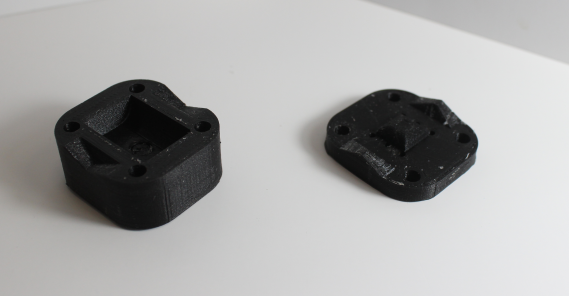
\includegraphics[width=0.9\textwidth]{Images/mold/mold.png}
        \caption{3D printed silicon mold, 1}
        \label{fig:mold}
    \end{subfigure}
    \begin{subfigure}{.45\linewidth}
        \centering
        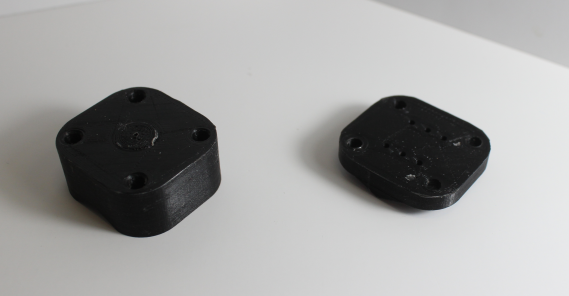
\includegraphics[width=0.9\textwidth]{Images/mold/moldinverted.png}
%    
\includegraphics[width=.4\textwidth]{Images/placeholder.png}
        \caption{Mold, 2}
        \label{fig:MoldInverted}
    \end{subfigure}
    \begin{subfigure}{.45\linewidth}
        \centering
%    
\includegraphics[width=.4\textwidth]{Images/placeholder.png}       
    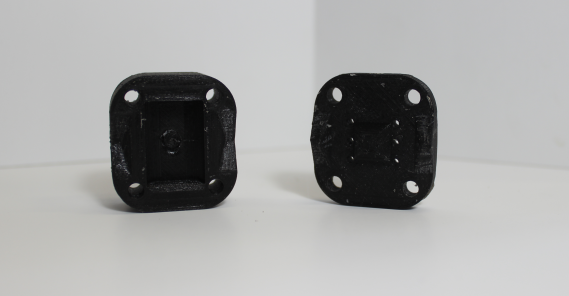
\includegraphics[width=0.9\textwidth]{Images/mold/moldstanding.png}
        \caption{Mold, 3}
        \label{label:MoldStanding}
    \end{subfigure}
    \begin{subfigure}{.45\linewidth}
        \centering
        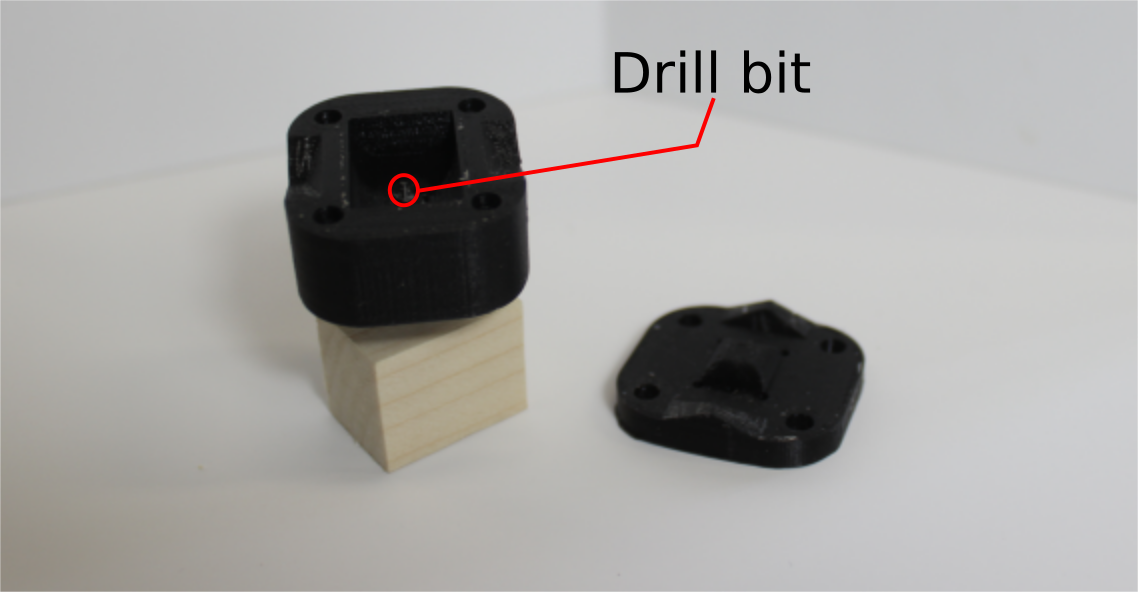
\includegraphics[width=0.9\textwidth]{Images/mold/drillinserted.png}          
%    
\includegraphics[width=.4\textwidth]{Images/placeholder.png} 
        \caption{Drillbit in place}
        \label{label:drillInserted}
    \end{subfigure}
    \begin{subfigure}{.45\linewidth}
        \centering
        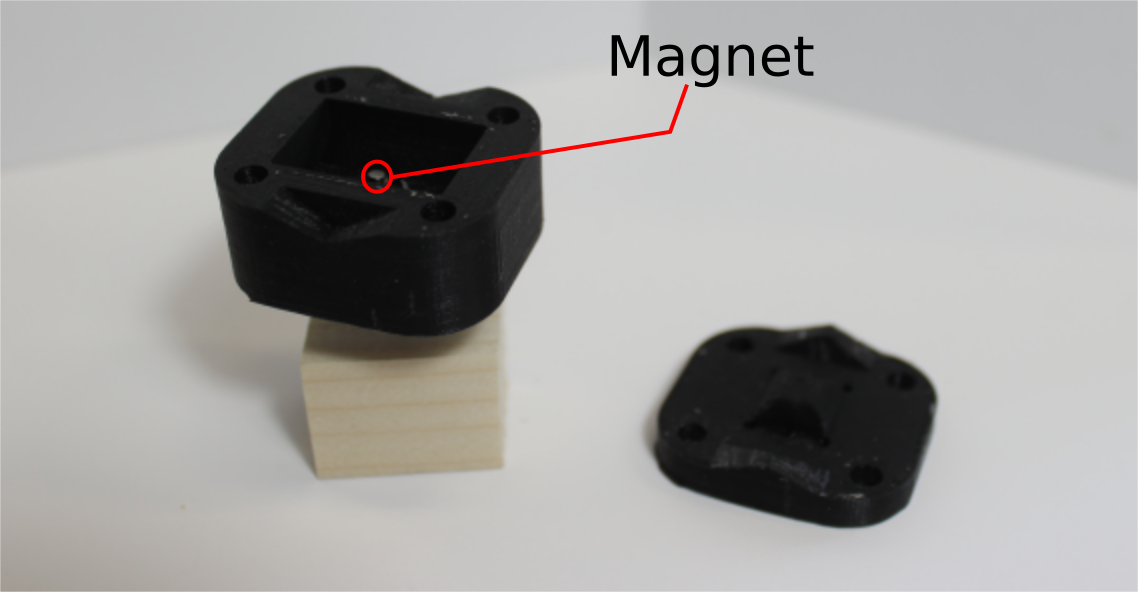
\includegraphics[width=0.9\textwidth]{Images/mold/withmagnet.png}       
  %  
\includegraphics[width=.4\textwidth]{Images/placeholder.png}
        \caption{Magnet in place}
        \label{fig:withmagnet}
    \end{subfigure}
    \begin{subfigure}{.45\linewidth}
        \centering
        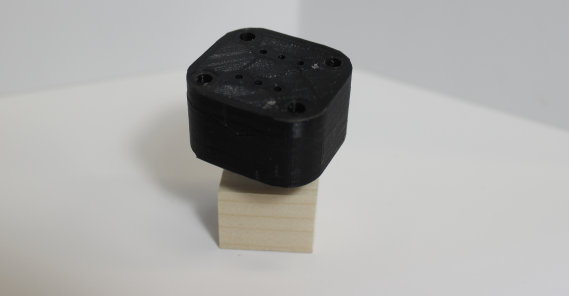
\includegraphics[width=0.9\textwidth]{Images/mold/closed.png}    
  %  
\includegraphics[width=.4\textwidth]{Images/placeholder.png}
        \caption{Mold closed}
        \label{fig:closed}
    \end{subfigure}    
    \begin{subfigure}{.45\linewidth}
        \centering
        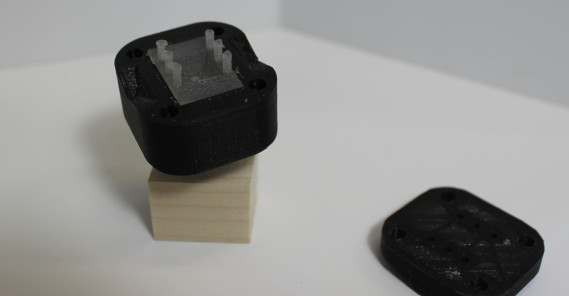
\includegraphics[width=0.9\textwidth]{Images/mold/withsilicon.png}       
  %  
\includegraphics[width=.4\textwidth]{Images/placeholder.png}
        \caption{Resulting silicon}
        \label{fig:withSilicon}
    \end{subfigure}
    \begin{subfigure}{.45\linewidth}
        \centering
        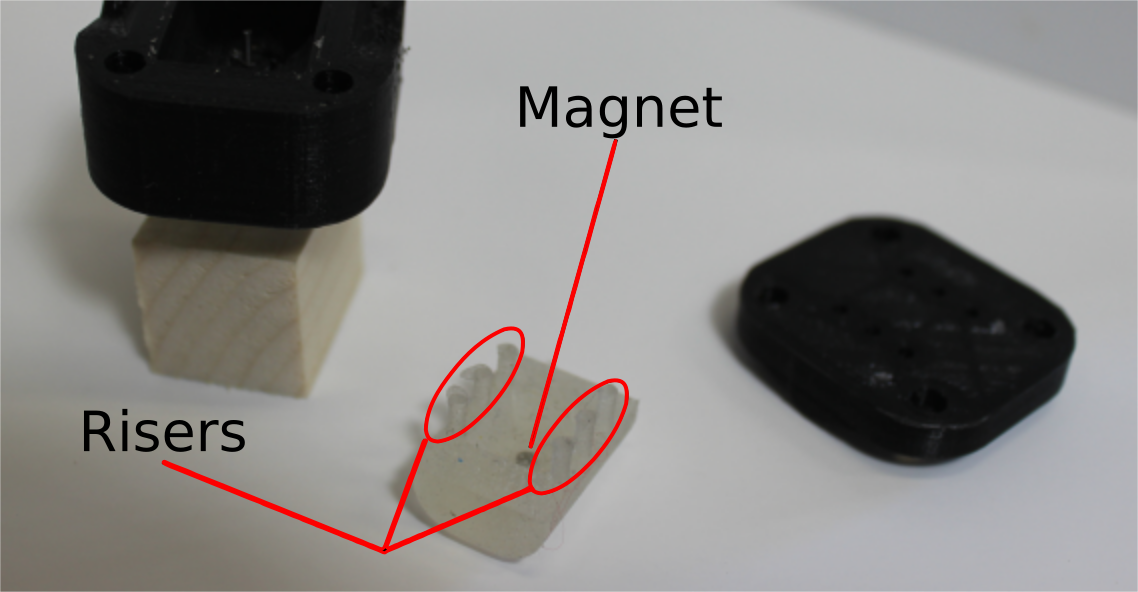
\includegraphics[width=0.9\textwidth]{Images/mold/complete.png}    
  %  
\includegraphics[width=.4\textwidth]{Images/placeholder.png}
        \caption{Complete, 1}
        \label{fig:complete}
    \end{subfigure}
    \begin{subfigure}{.45\linewidth}
        \centering
        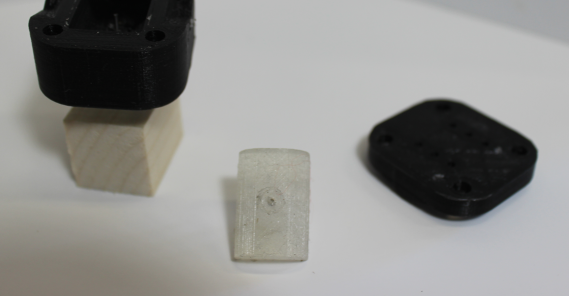
\includegraphics[width=0.9\textwidth]{Images/mold/complete2.png}    
  %  
\includegraphics[width=.4\textwidth]{Images/placeholder.png}
        \caption{Complete, 2}
        \label{fig:complete2}
    \end{subfigure}
    \caption{Images of the mold and molding process}
    \label{figure:Molding}
\end{figure}


